\chapter{Results}
\label{ch:testing}

\section{Simulation data}
In our testing we ran the simulation from 200 to over 1000 iterations, as there was no significant difference from 200 to 1000 iterations we did most of the simulations to 200 iterations.

The number of passengers was set to the ship maximum number of passengers stated on Cruisedeckplans LLC\cite{cruseships} website.

The hazards on-board the ship was set to increase at every second time step, both in number of nodes and how deadly it was in a particular node. In ACO, at each time step, the passengers was set to use 200 ants to find their way trough the ship, and each ant holding 200 pheromones to spread around. Also in each of these simulation, one fire was started, however some times it was randomly chosen one to three times.

In some of our simulation, it happens that a passenger would walk on board the ship for much longer then 300 time steps. However we have cut the graph at 300 time steps, as this would show more details in the graph about the algorithms and the average number of survives past 300 did not change.


\subsection{Celebrity Xpedition}


in these first two figures, \ref{fig:celebSafestDF} and \ref{fig:celebShortestDF}, Dijkstra was only run once at the start of the simulation. This yielded some unexpected results. First of when looking for the safest path when as we expected that ACO would outperform Dijkstra. However when looking for the shortest path, ACO started out good but Dijkstra pulled ahead after about 100 time steps. This may be explained that ACO started taking more risk-full paths to try to keep the passengers not clogging each other up.


\begin{figure} [h]
\centering
\hspace*{-1.0in}
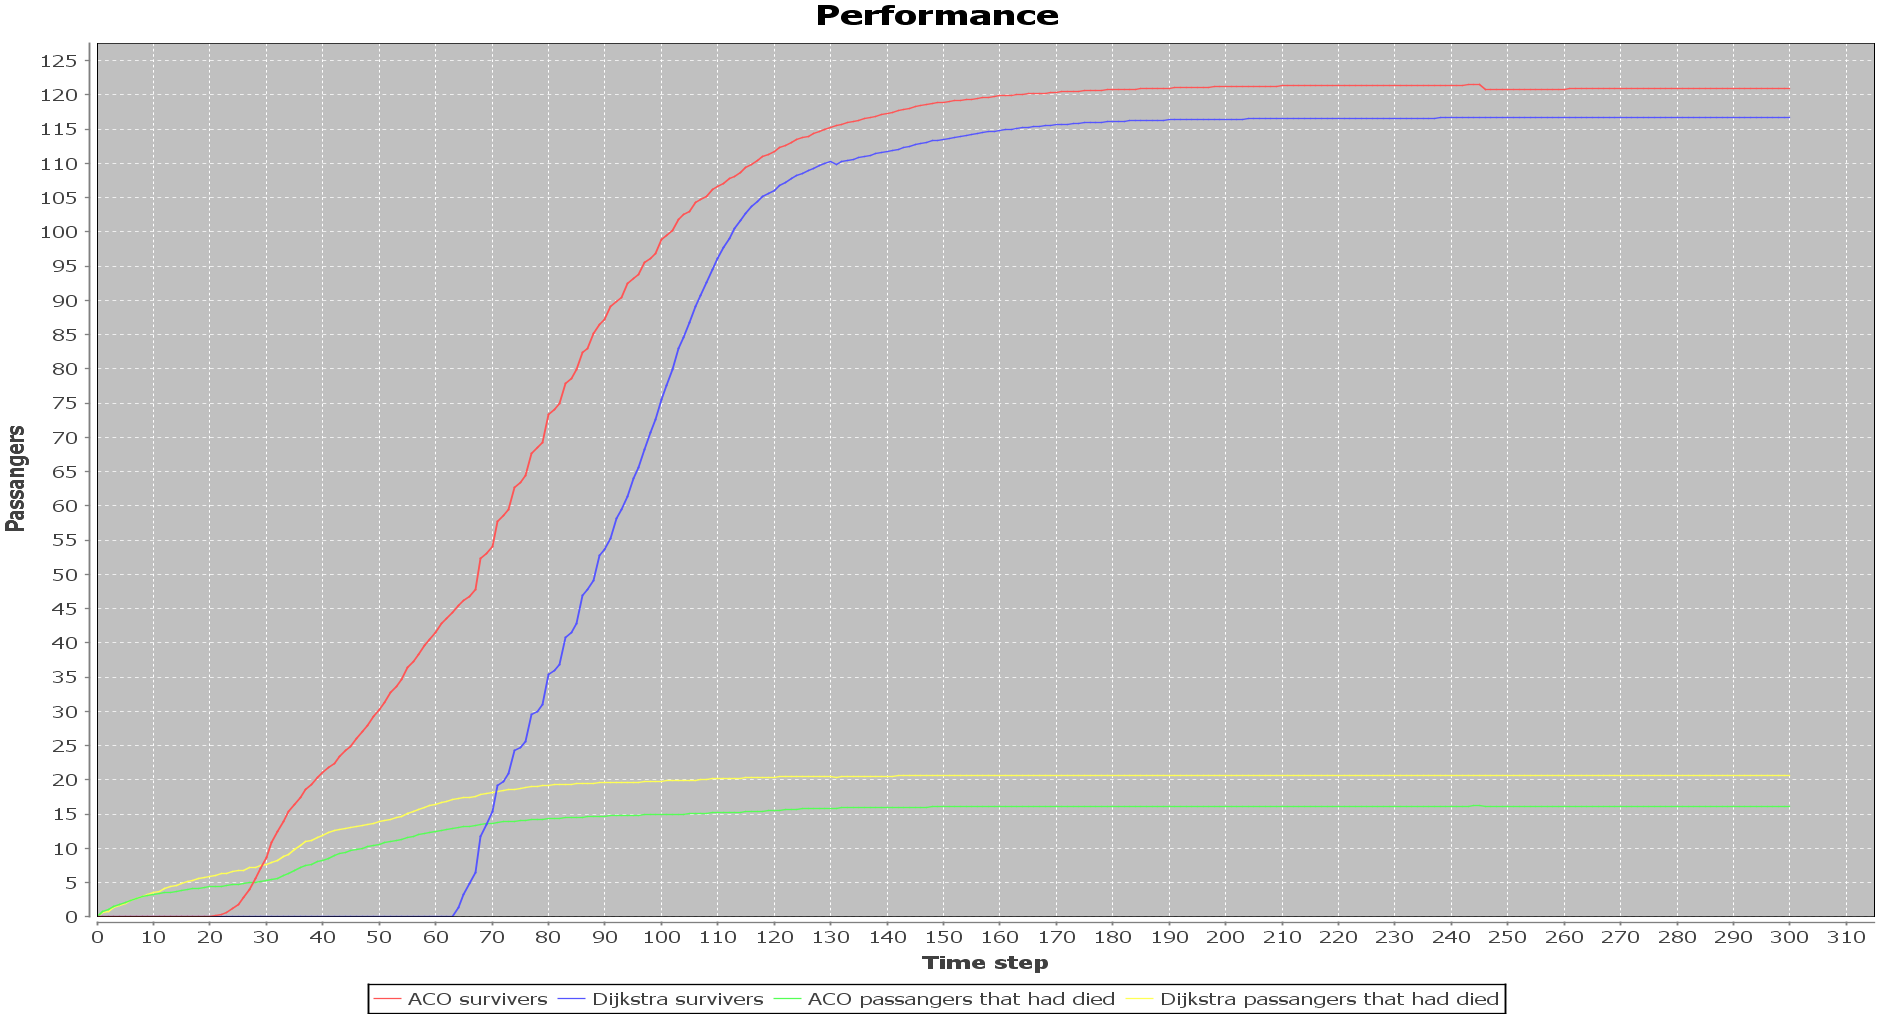
\includegraphics[scale=0.35]{images/Graph-using-1000-rounds-140-passangers-safestpath-and-one-fire-dijkstra-one-time.png}
\caption{Taking safest path with Dijkstra only running at start.}
\label{fig:celebSafestDF}
\end{figure}

\begin{figure} [h]
\centering
\hspace*{-1.0in}
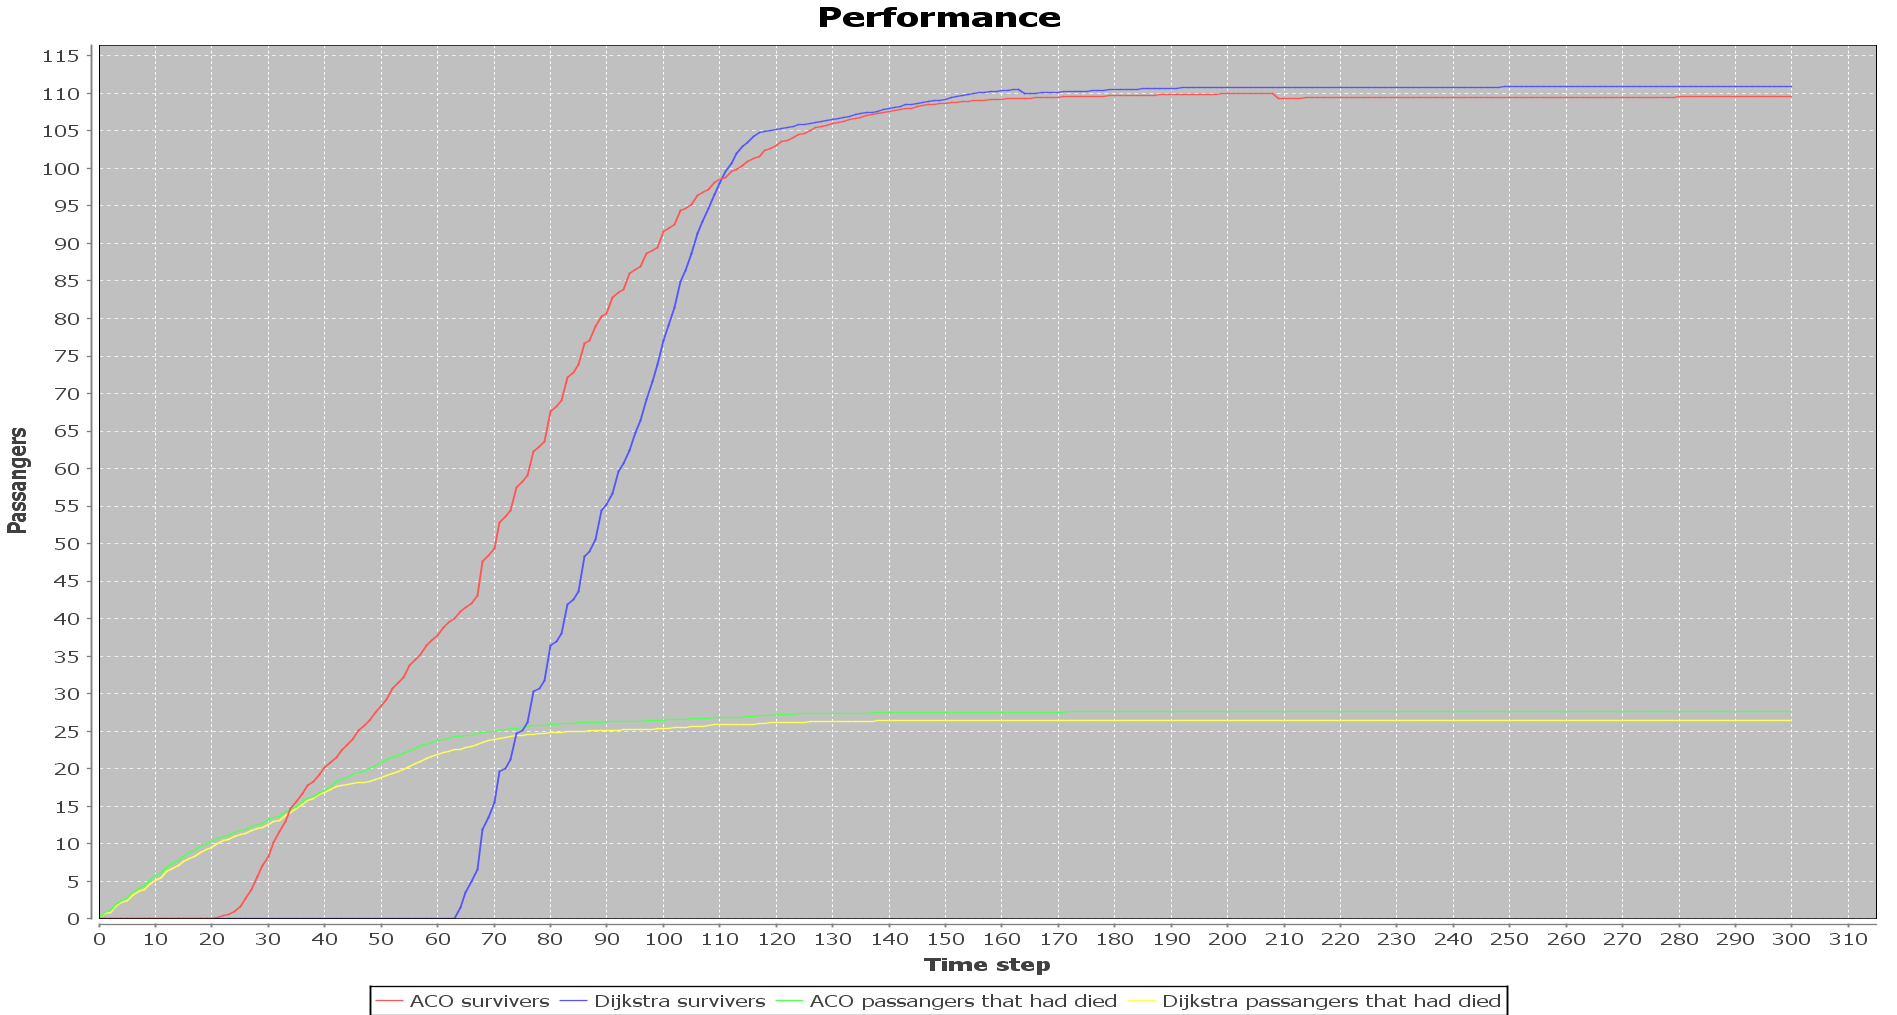
\includegraphics[scale=0.35]{images/Graph-using-1000-rounds-140-passangers-shortestpath-and-one-fire-dijkstra-one-time.png}
\caption{Taking shortest path with Dijkstra only running at start.}
\label{fig:celebShortestDF}
\end{figure}


In \ref{fig:celebShortest} you can see how well the different algorithms did. In both cases we only used one hazard(Fire) that spread on board the ship. As shown in the graph, Dijkstra outperforms ACO in both early and late stages of this graph. In the beginning there are more passengers dying to ACO chosen path then there is in Dijkstra's chosen path, a good sign that both are finding different paths. As shortest path is measured in shortest time needed rather then shortest way to exit, it may be that Dijkstra spread the passengers more out then ACO.

Even when more passengers are dying at the beginning of the simulations, they both have the same boost in saved passengers at each time step.

The biggest problem for ACO over Dijkstra is avoiding the hazards. Shown in the graph you can see that the death toll for ACO increases faster then Dijkstra's death toll.

\begin{figure} [h]
\centering
\hspace*{-1.0in}
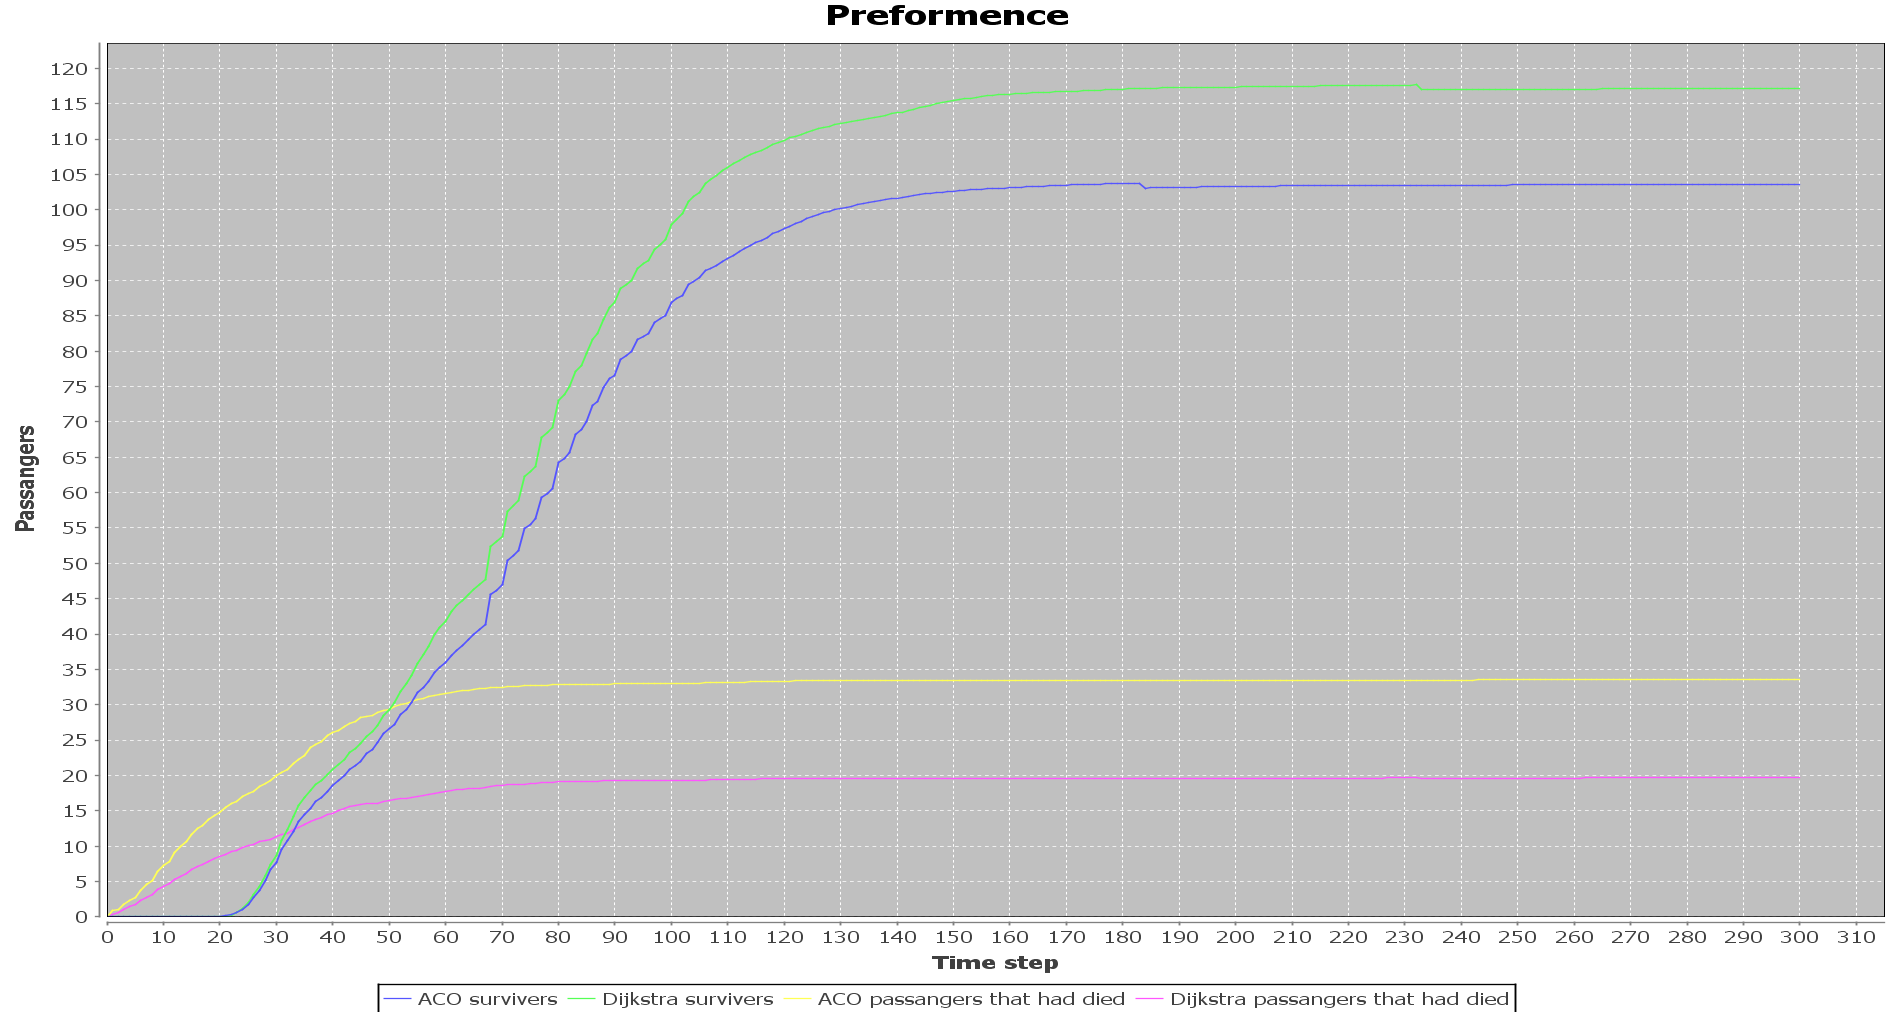
\includegraphics[scale=0.35]{images/Graph-using-200-rounds-140-passangers-and-shortest-first-one-hazzard.png}
\caption{Taking shortest path.}
\label{fig:celebShortest}
\end{figure}

In \ref{fig:celebSafty}, we are using the same parameters as the first one, only difference is that we are looking after the safest path rather then the shortest path for the passengers. It is clearly shown that the death toll on the passengers is far lower then the previous one.
However Dijkstra proves yet again to outperform ACO in this instance. After about 30 time steps Dijkstra starts to pull ahead of ACO in number of passengers it have guided to the lifeboats. Even in number of deaths it is shown that Dijkstra is better at avoiding them.

If you look at Dijkstra in both cases, the number of deaths when looking after the safest path is 50\% less when looking for the shortest path.

As mention earlier that the number of rounds above 200 did not matter may be shown in the two graphs below, both of them have the same set of parameters, only to have 1000 iteration instead of 200.

\begin{figure} [h]
\centering
\hspace*{-1.0in}
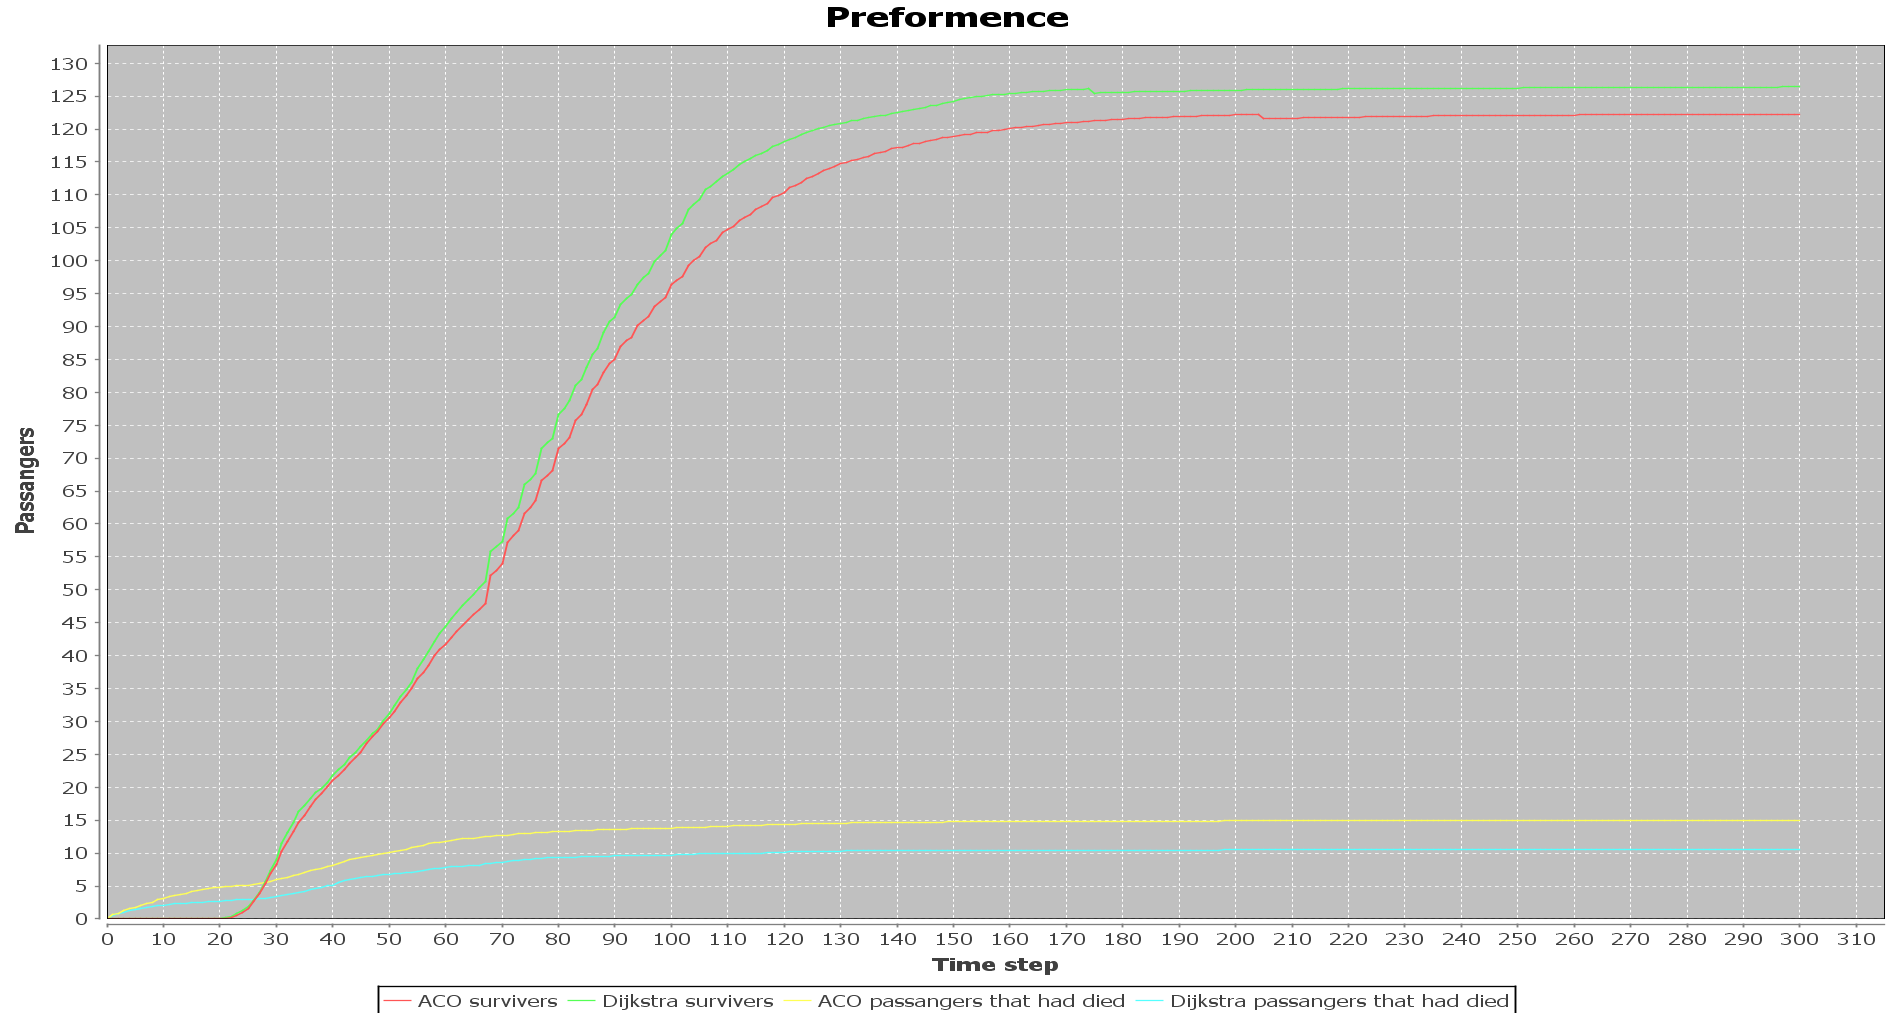
\includegraphics[scale=0.35]{images/Graph-using-200-rounds-140-passangers-and-safest-first-one-hazzard.png}
\caption{Taking safest path.}
\label{fig:celebSafty}
\end{figure}


\ref{fig:celebSafty1000round} is 1000 iterations of the simulation with same parameters as \ref{fig:celebSafty}, and is going for the safest route for the passengers. Now in \ref{fig:celebShort1000round} we did the exact same thing, only we changed the algorithms to look for the shortest path rather then safest.

\begin{figure} [h]
\centering
\hspace*{-1.0in}
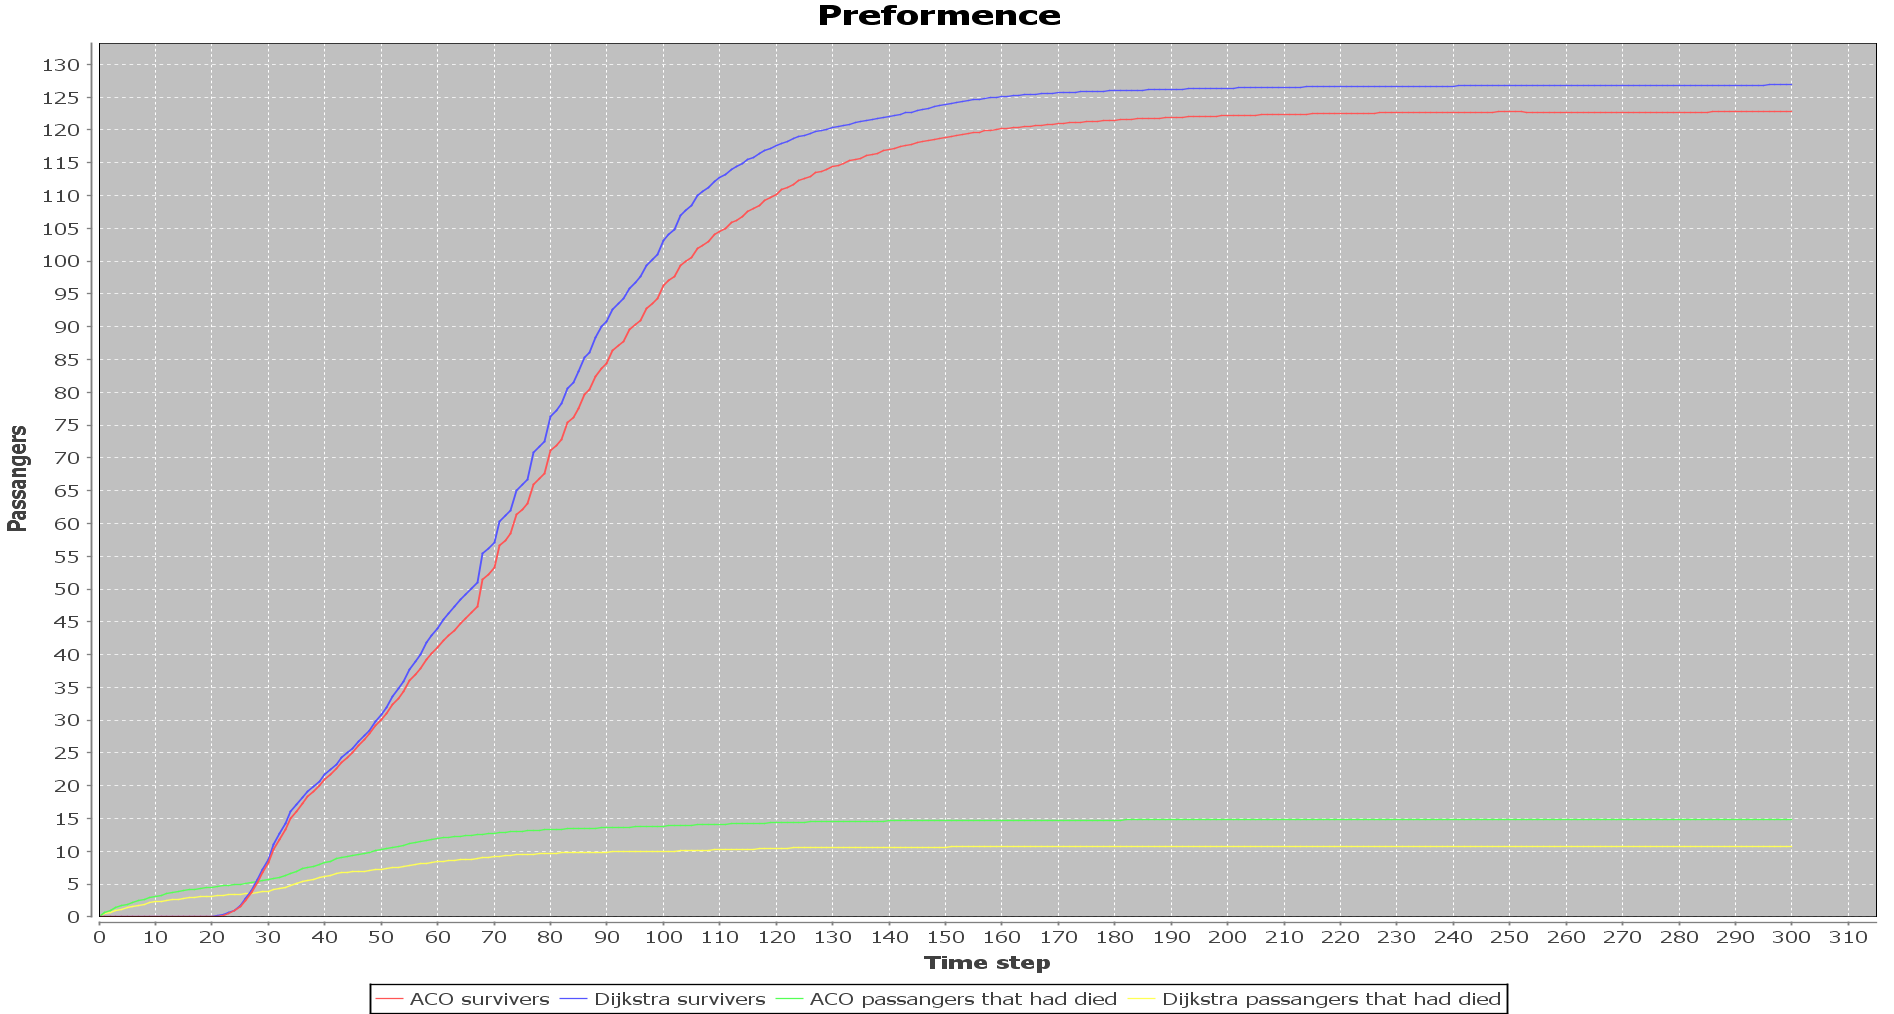
\includegraphics[scale=0.35]{images/Graph-using-1000-rounds-140-passangers-safest-path-and-one-fire.png}
\caption{Taking safest path with 1000 iterations.}
\label{fig:celebSafty1000round}
\end{figure}

\begin{figure} [h]
\centering
\hspace*{-1.0in}
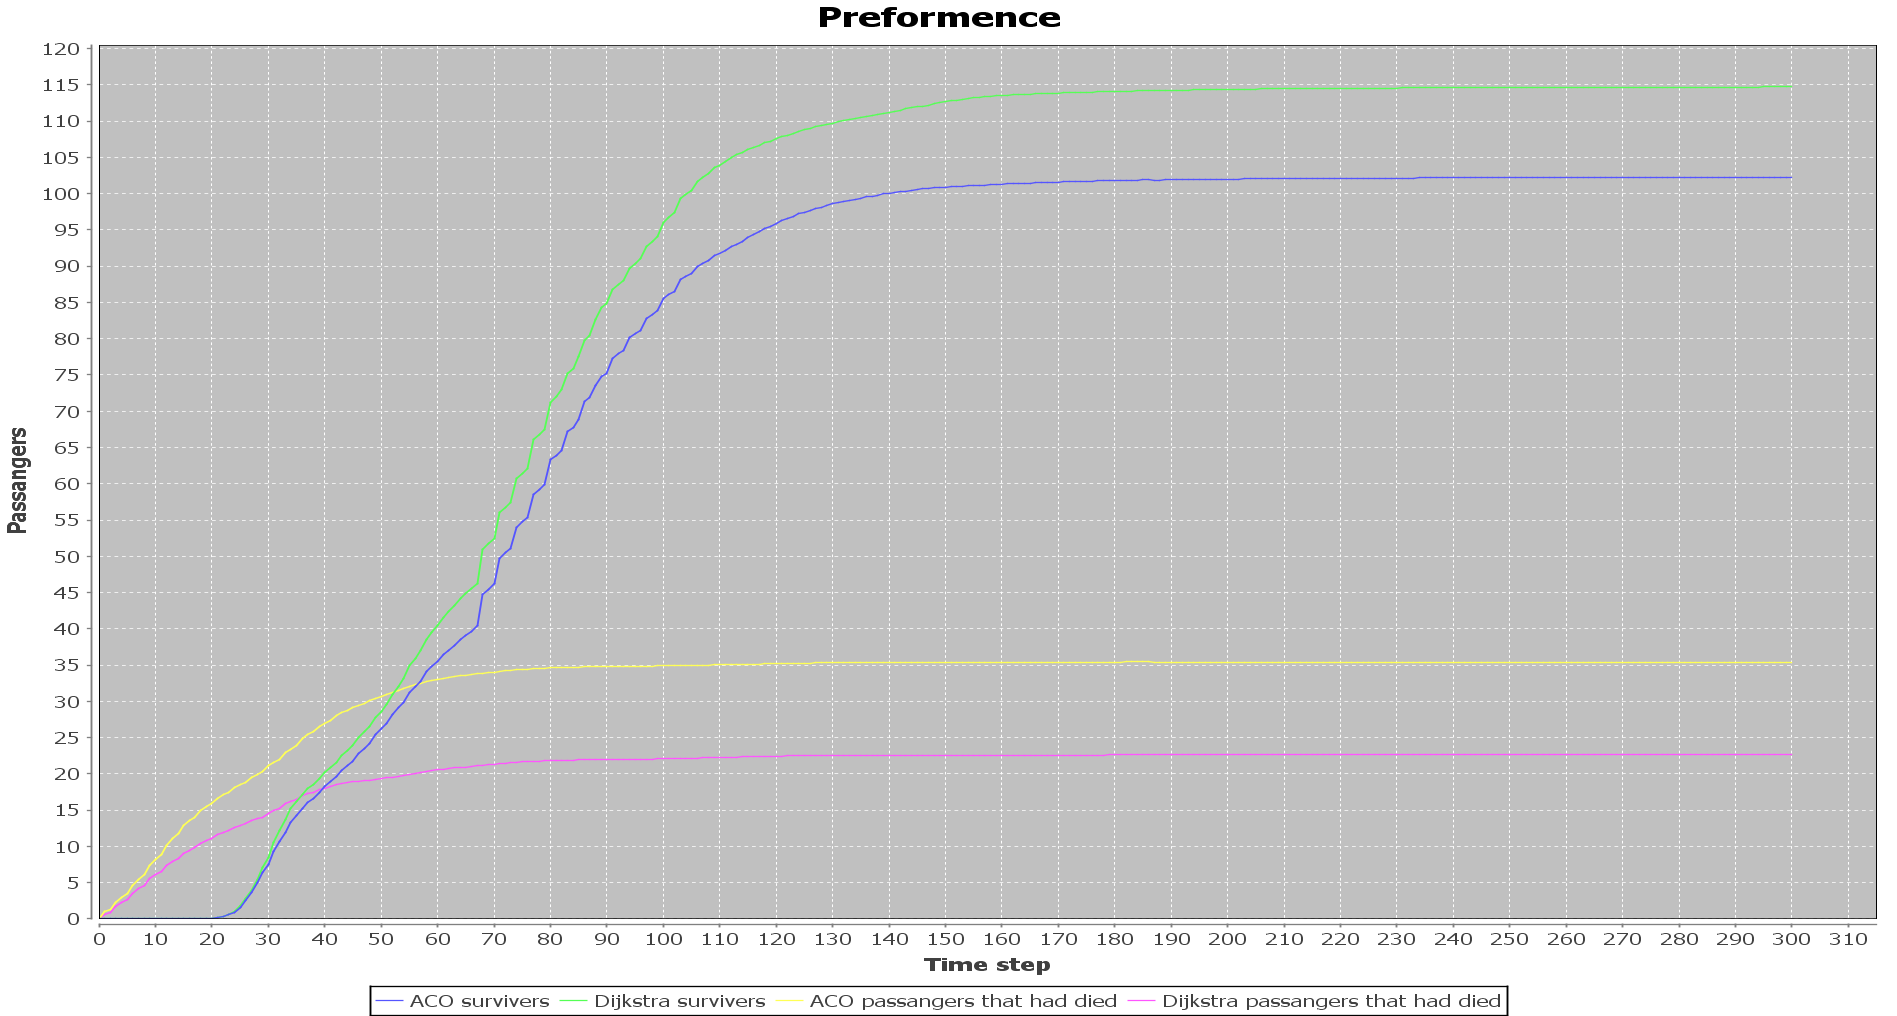
\includegraphics[scale=0.35]{images/Graph-using-1000-rounds-140-passangers-shortest-path-and-one-fire.png}
\caption{Taking shortest path with 1000 iterations.}
\label{fig:celebShort1000round}
\end{figure}


In \ref{fig:celebShortPherInEdges} and \ref{fig:celebSafePherInEdges} we tested what would the difference be if we used pheromones in edges rather then in the node themselves, this showed that the ACO preformed better then our other simulations. It was compared to Dijkstra to control that there was not something special happening. The main difference is when looking for the shortest path rather then the safest. When looking for the safest there are only some small difference in both simulations.

\begin{figure} [h]
\centering
\hspace*{-1.0in}
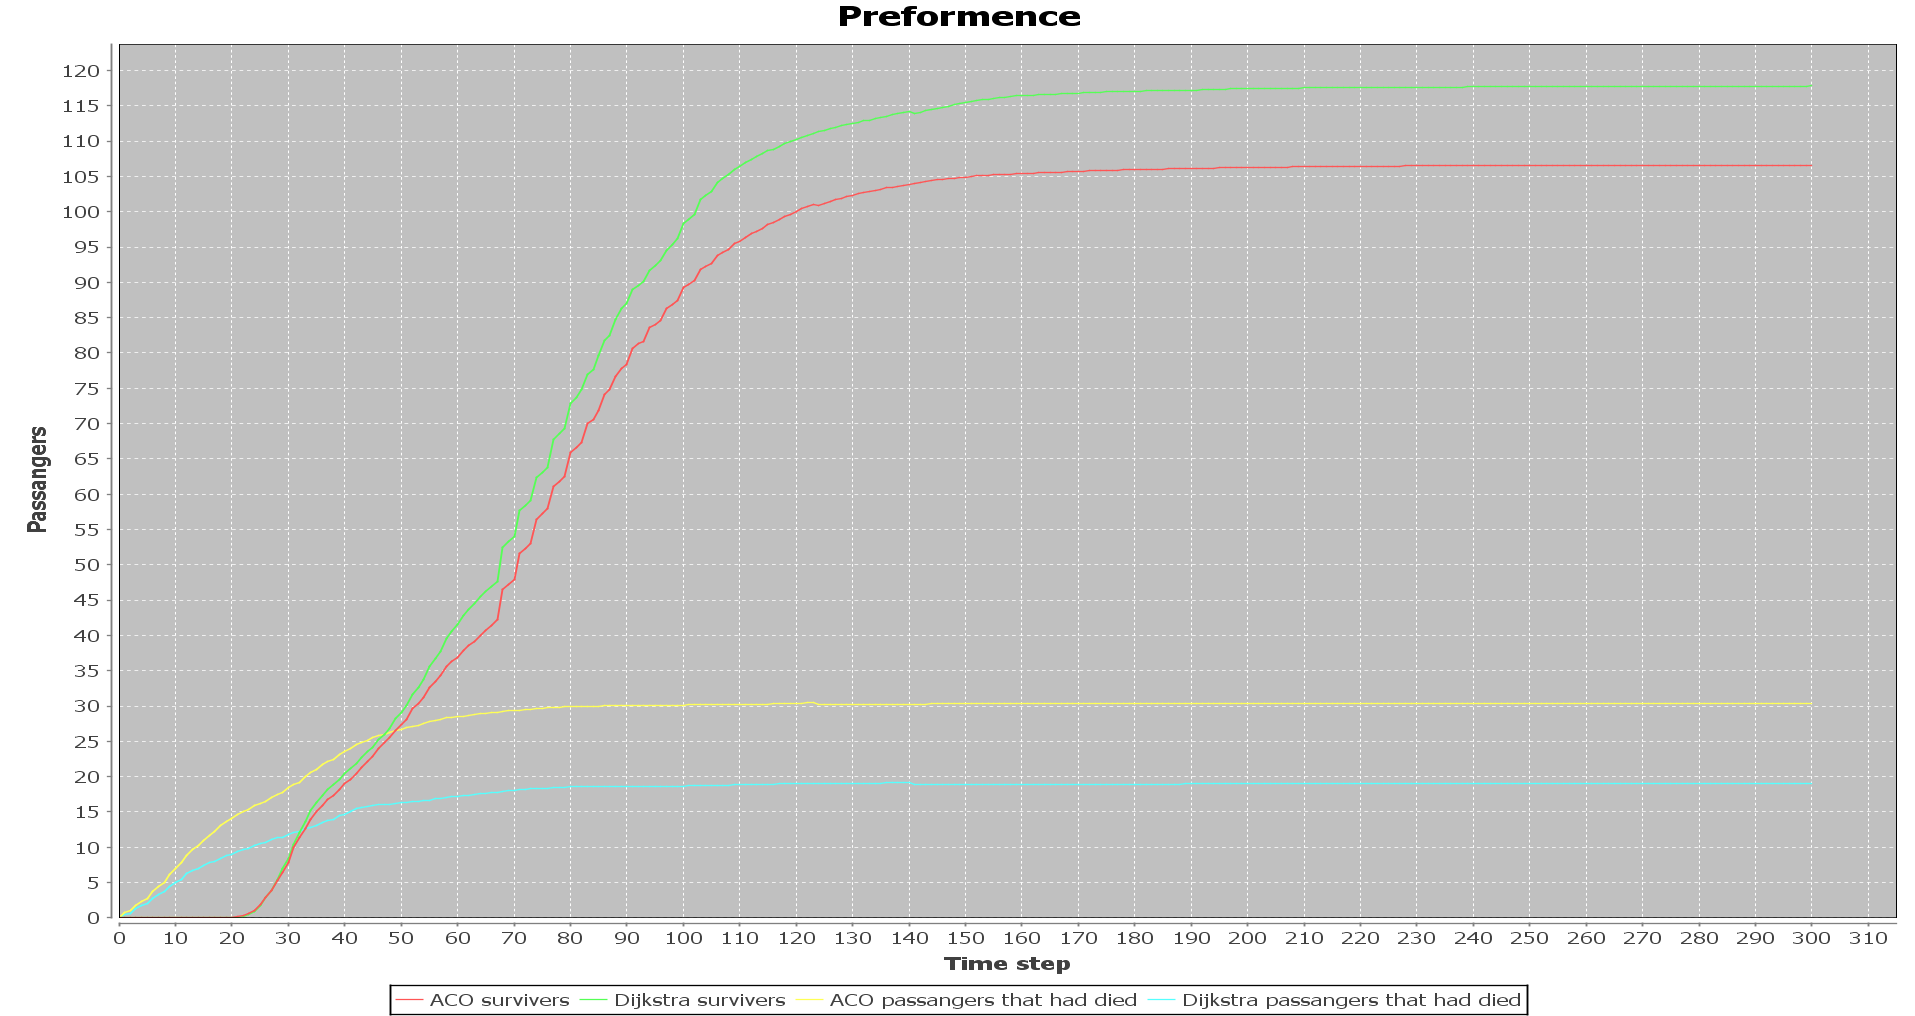
\includegraphics[scale=0.35]{images/Graph-using-200-rounds-140-passangers-and-shortest-first-one-hazzard-and-ACO-having-pheremons-in-edges.png}
\caption{Taking shortest path with pheromones in edges.}
\label{fig:celebShortPherInEdges}
\end{figure}

\begin{figure} [h]
\centering
\hspace*{-1.0in}
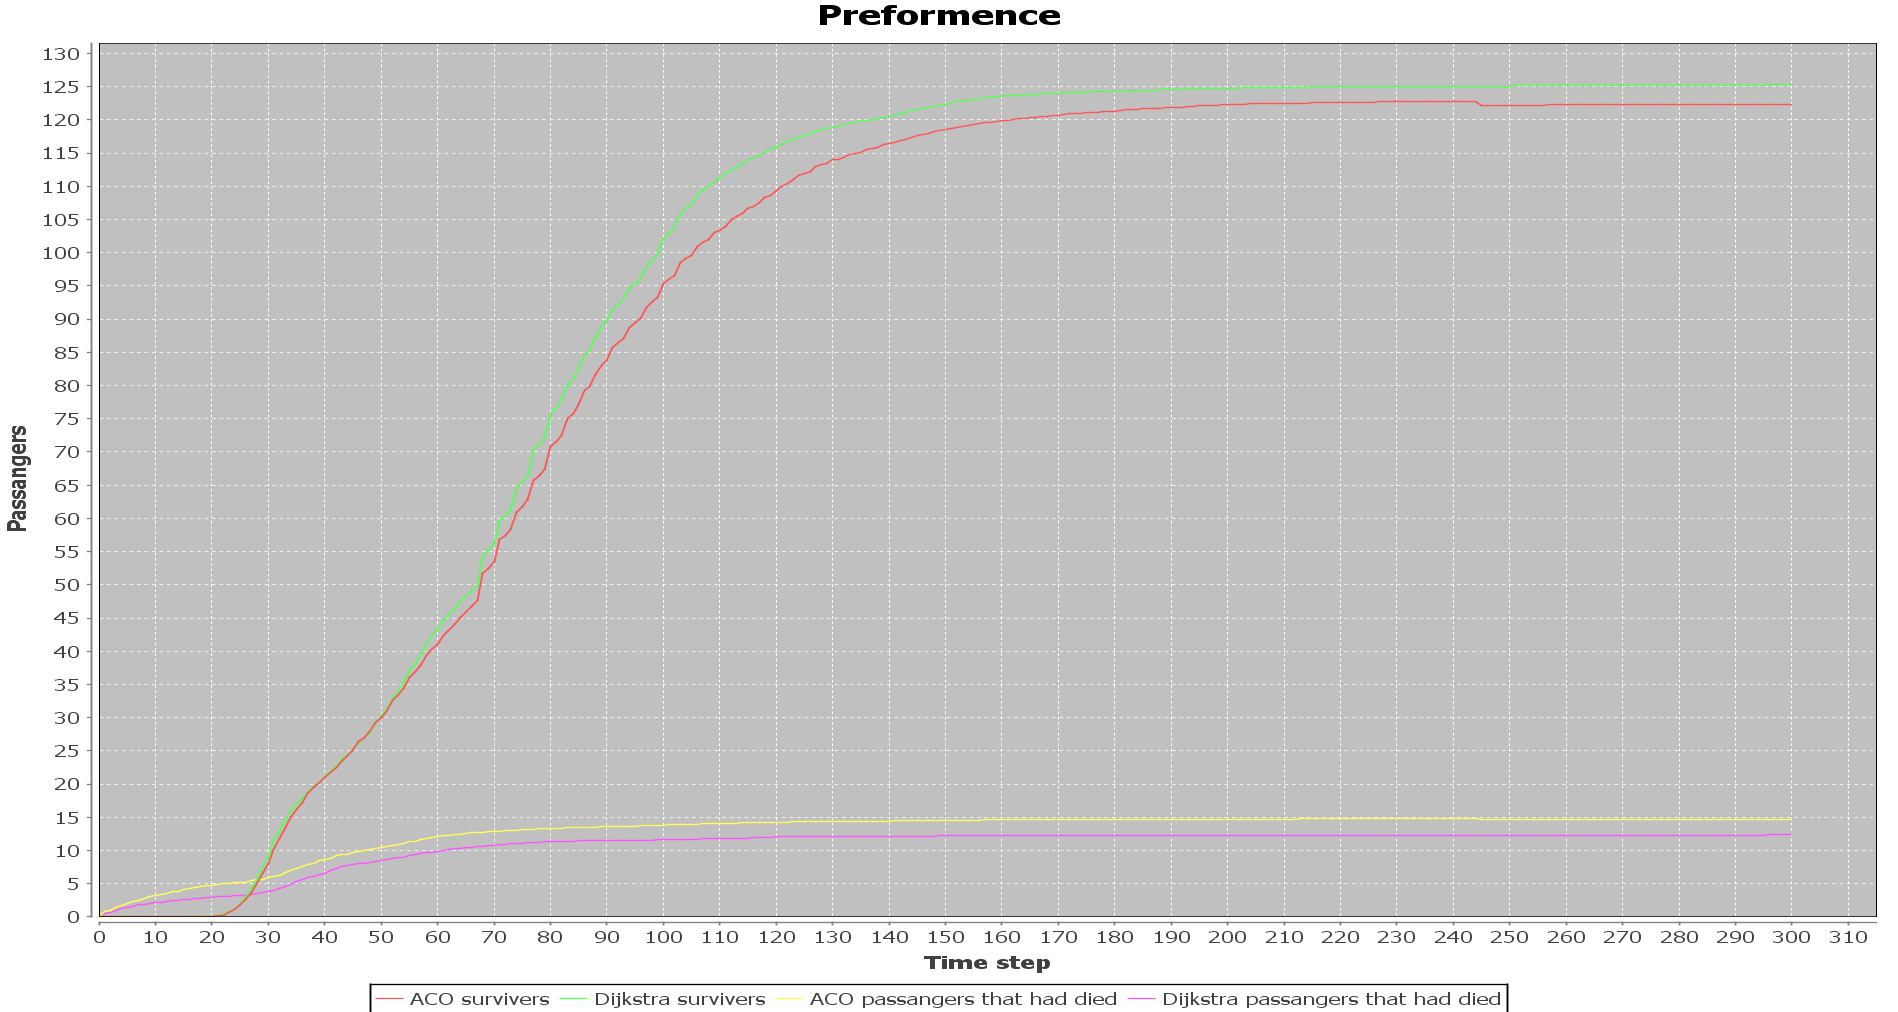
\includegraphics[scale=0.35]{images/Graph-using-200-rounds-140-passangers-and-safest-first-one-hazzard-and-ACO-having-pheremons-in-edges.png}
\caption{Taking safest path with pheromones in edges.}
\label{fig:celebSafePherInEdges}
\end{figure}


When the chance of panic changed to a higher chance both algorithms struggled more to guide the passengers to safety. Dijkstra took the hit hardest as it sometimes it would send it one direction, then panic and go back, therefore taking a long time before that passenger got to safety or died. However it was also Dijkstra that preformed best overall, shown in \ref{fig:celebShortHPanic} and \ref{fig:celebSafeHpanic}.

\begin{figure} [h]
\centering
\hspace*{-1.0in}
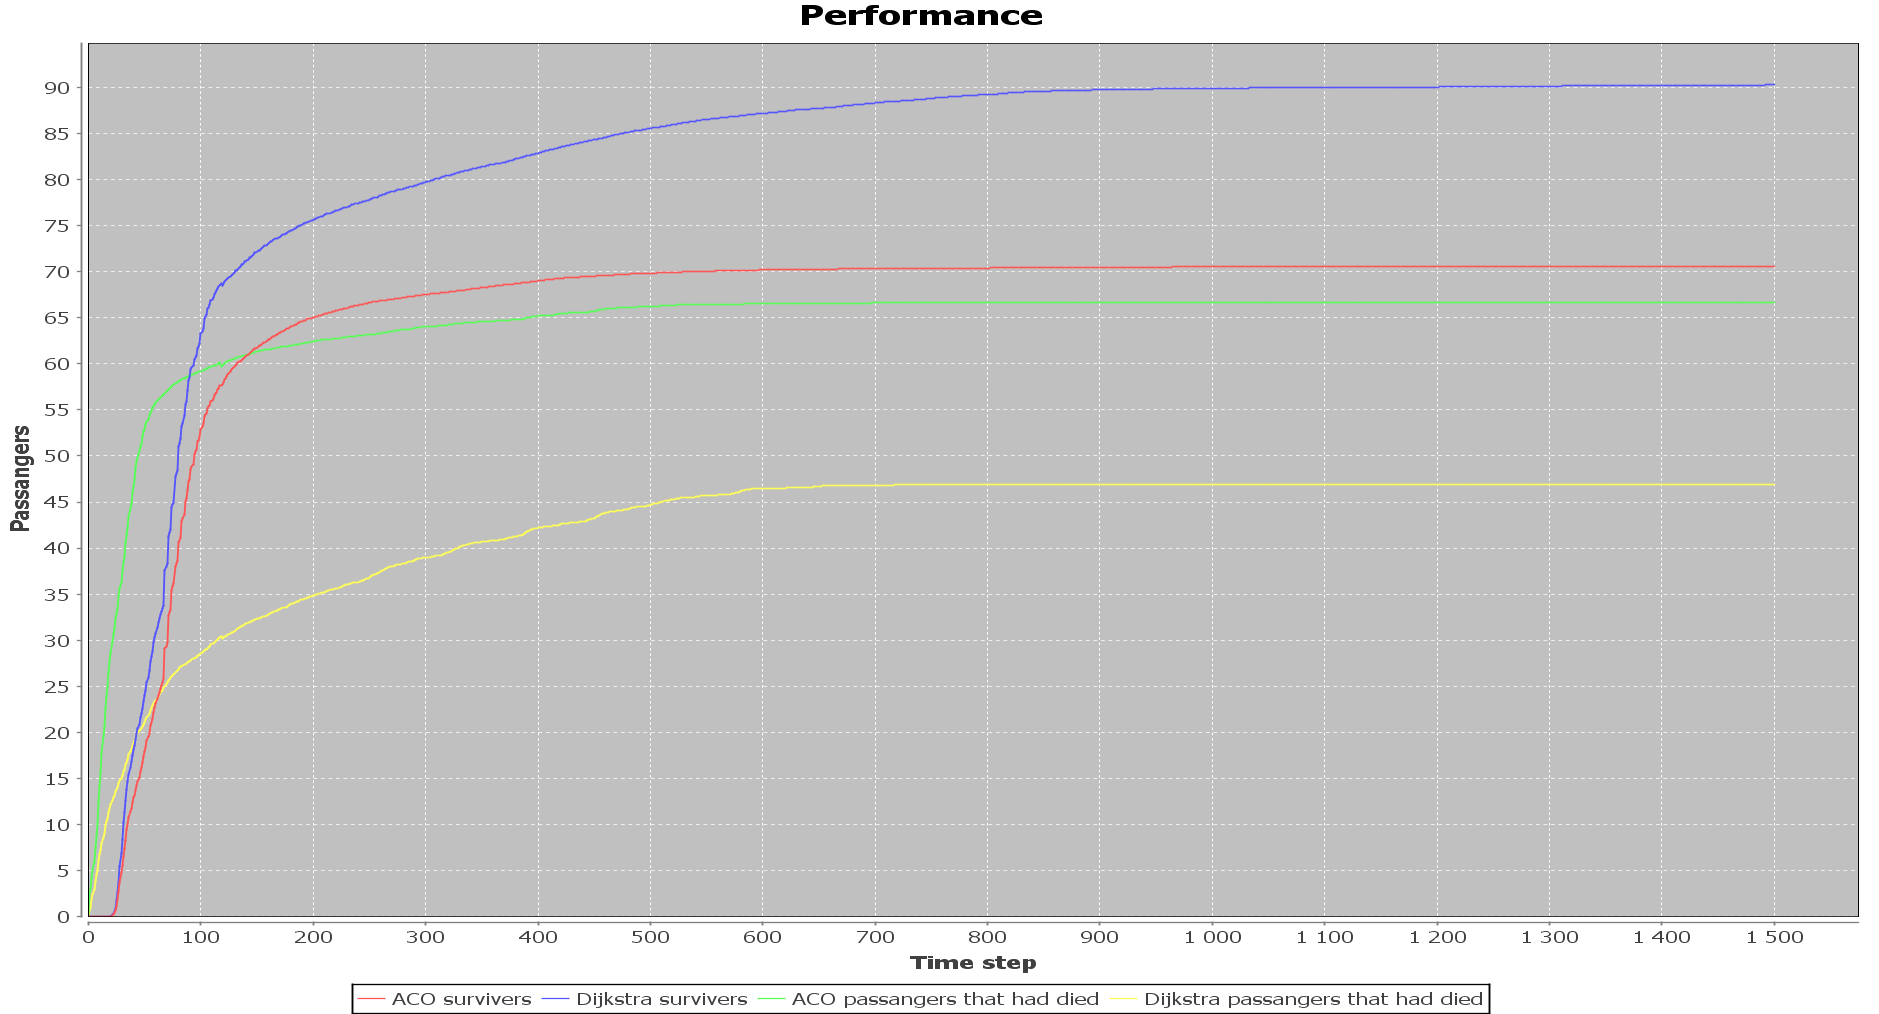
\includegraphics[scale=0.35]{images/Graph-using-1000-rounds-140-passangers-shortestpath-and-one-fire-high-panic.png}
\caption{Taking shortest path with pheromones in edges.}
\label{fig:celebShortHPanic}
\end{figure}

\begin{figure} [h]
\centering
\hspace*{-1.0in}
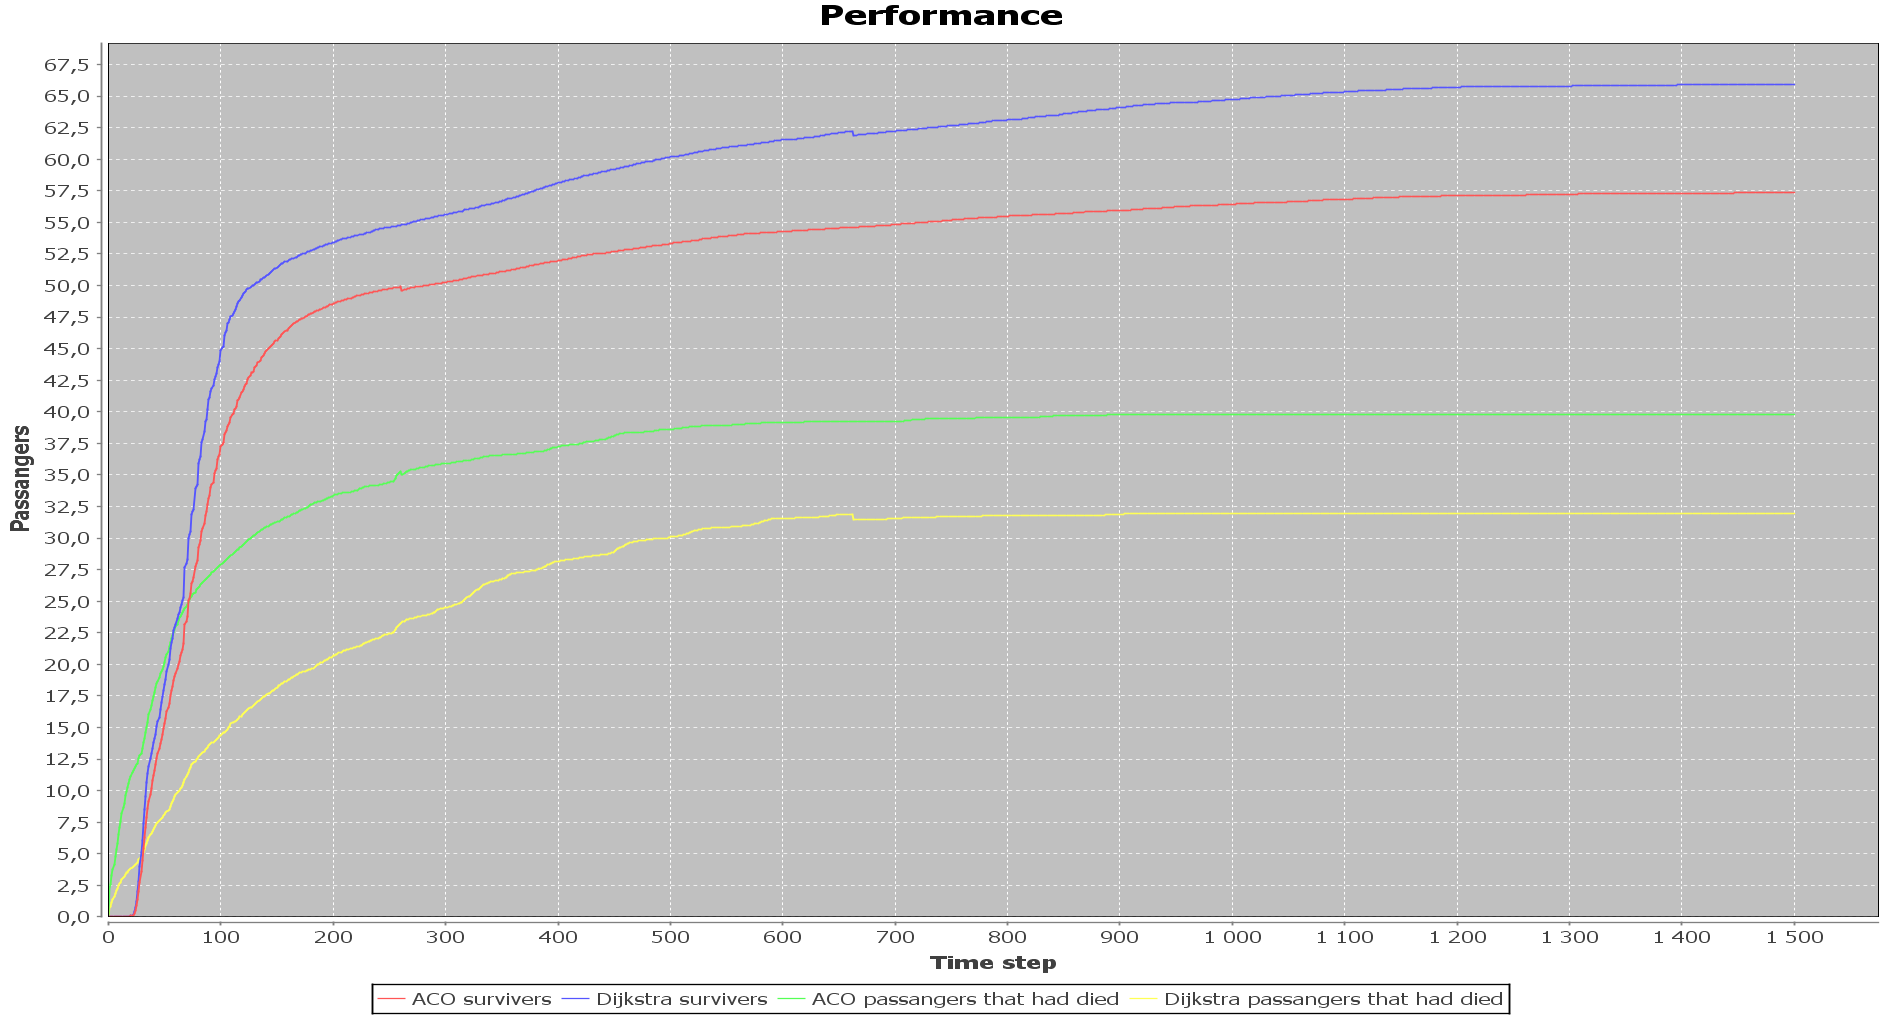
\includegraphics[scale=0.35]{images/Graph-using-1000-rounds-140-passangers-safestpath-and-one-fire-high-panic.png}
\caption{Taking safest path with pheromones in edges.}
\label{fig:celebSafeHpanic}
\end{figure}
